%%%%%%%%%%%%%%%%%%%%%%%%%%%%%%%%%%%%%%%%%
% Short Sectioned Assignment
% LaTeX Template
% Version 1.0 (5/5/12)
%
% This template has been downloaded from:
% http://www.LaTeXTemplates.com
%
% Original author:
% Frits Wenneker (http://www.howtotex.com)
%
% License:
% CC BY-NC-SA 3.0 (http://creativecommons.org/licenses/by-nc-sa/3.0/)
%
%%%%%%%%%%%%%%%%%%%%%%%%%%%%%%%%%%%%%%%%%

%----------------------------------------------------------------------------------------
%	PACKAGES AND OTHER DOCUMENT CONFIGURATIONS
%----------------------------------------------------------------------------------------

\documentclass[paper=a4, fontsize=11pt]{scrartcl} % A4 paper and 11pt font size

\usepackage{mathpazo}
\usepackage{placeins}
\usepackage[T1]{fontenc} % Use 8-bit encoding that has 256 glyphs
\usepackage{fourier} % Use the Adobe Utopia font for the document - comment this line to return to the LaTeX default
\usepackage[english]{babel} % English language/hyphenation
\usepackage{amsmath,amsfonts,amsthm} % Math packages
\usepackage{listings}
\usepackage{amssymb}
\usepackage{graphicx}
\graphicspath{ {/home/poulastya/Documents/Assignments/Neural Network/git_as/ex5} }

\usepackage{sectsty} % Allows customizing section commands
\allsectionsfont{\raggedright \normalfont} % Make all sections centered, the default font and small caps

\usepackage{fancyhdr} % Custom headers and footers
\pagestyle{fancyplain} % Makes all pages in the document conform to the custom headers and footers
\fancyhead{} % No page header - if you want one, create it in the same way as the footers below
\fancyfoot[L]{} % Empty left footer
\fancyfoot[C]{} % Empty center footer
\fancyfoot[R]{\thepage} % Page numbering for right footer
\renewcommand{\headrulewidth}{0pt} % Remove header underlines
\renewcommand{\footrulewidth}{0pt} % Remove footer underlines
\setlength{\headheight}{9pt} % Customize the height of the header
\setlength{\textheight}{640pt} % Customize the height of the header

\setlength\parindent{0pt} % Removes all indentation from paragraphs - comment this line for an assignment with lots of text

%----------------------------------------------------------------------------------------
%	TITLE SECTION
%----------------------------------------------------------------------------------------

\newcommand{\horrule}[1]{\rule{\linewidth}{#1}} % Create horizontal rule command with 1 argument of height

\title{	
\normalfont \normalsize 
\textsc{Bonn-Rhein-Sieg University of Applied Sciences \\Department of Computer Science\\Neural Networks} \\ [10pt] % Your university, school and/or department name(s)
\horrule{0.5pt} \\[0.4cm] % Thin top horizontal rule
\LARGE  Exercise 5\\ % The assignment title
\horrule{2pt} \\[0.5cm] % Thick bottom horizontal rule
}
\date{}
\author{Poulastya Mukherjee, Benjamin Thompson} % Your name

\begin{document}

\maketitle % Print the title

%----------------------------------------------------------------------------------------
%	PROBLEM 1
%----------------------------------------------------------------------------------------

\section{Read Chapter 3.1-3.5 from Haykin's book; summarize or sketch your insights in mind-map or
an outline or a summary.}

\begin{itemize}
\item Rosenblatt proved that given linearly separable data, a perceptron is proven to converge.
\item Least mean square algorithm is the backbone of linear adaptive filters
\item Adaptive filtering
\subitem m dimensional input produces scalar output
\subitem data equally distributed
\subitem data can be spread over space (snapshot) or over time (uniformly spaced in time)
\subitem Filtering process produces the output and error signals
\subitem Adaptive process involves adjustments based on errors
\subitem Error correction is an optimization problem
\item Unconstrained optimization techniques
\subitem Optimal solution is gradient of cost function equal to 0
\item Steepest descent
\subitem converges slowly
\subitem size of eta produces overdamped response when small, under when large
\item Newton method
\subitem needs to be twice continuously differentiable wrt w to form hessian
\subitem converges quickly and generally not subject to underdamped behavior of steepest descent
\subitem Needs to be positive definite matrix, however there is no gaurantee of that.
\item Gauss Newton method
\subitem Only requires jacobian of the error vector as opposed to hessian of cost function
\subitem Jacobian product must be non singular
\item Least mean squares
\subitem Inverse of the learning rate eta is the 
\subitem weight vector traverses random trajectory in contrast with steepest descent
\subitem The stability of the system is determined by choosing an appropriate eta for x
\subitem Model independent, therefore robust
\subitem Needs approx 10x the dimensionality iterations to converge
\end{itemize}

\section{ (3.1) }
\[\varepsilon (w) = \frac{1}{2}.\sigma^{2} -r_{xd}.w + \frac{1}{2}r_{x}w^{2}\] \\
Calculating Descent
\[\bigtriangledown \varepsilon (w) = g = r_{x}w - r_{xd} \]\\
Applying Steepest Descent
\[w(n+1) = w(n) - \eta .g(n) \]\\ 
where g(n) is the gradient and $\eta$ is the learning rate
\[w(n+1) = w(n) - \eta .[r_{x}w(n) - r_{xd}]\] \\ 
By applying steepest descent we get the expression for the change in weight
\[\bigtriangleup w(n) = \eta .[r_{x}w(n) - r_{xd}]\]

%\FloatBarrier
%\begin{figure}[h]
%\centering
%\includegraphics[width=0.4\textwidth]{ex1_im1}
%\caption{Piece-wise linear activation function [Haykin]}
%\end{figure}
%\FloatBarrier

\section{ (3.2) }
\subsection{a}
\[w = \begin{bmatrix} w1\\ w2 \end{bmatrix}\] \\ 
\[w^{T} = \begin{bmatrix} w1 & w2 \end{bmatrix} \]\\ 
\[r_{xd} = \begin{bmatrix}

 0.8182\\ 0.354 \end{bmatrix} \]\\ 
\[R_{x} = \begin{bmatrix} 1 & 0.8182\\ 0.8182 & 1 \end{bmatrix}\] \\ 

\[\varepsilon(w) = \frac{1}{2}.\sigma^{2} - r^{T}_{xd}.w + \frac{1}{2}w^{T}R_{x}w\] \\
After calculating the gradient of the equation and equating it to 0 we get the optimal values of \\
$w^{*}$ as the point where the slope is zero is either minima or maxima
 \[\bigtriangledown \varepsilon (w) = \begin{bmatrix} -0.8182 + w1 + 0.8182w2\\ -0.354 + w1 + 0.8182w1 \end{bmatrix} = 0 \]\\
If we differentiate the above equation again using the gradient we will see that the resulting \\ matrix is same as R i.e. positive hence proving that the point we found is minima 
\[ w^{*} = \begin{bmatrix} 1.599\\ -0.95 \end{bmatrix}\]


\subsection{b}
\textbf{Code is provided at the end}


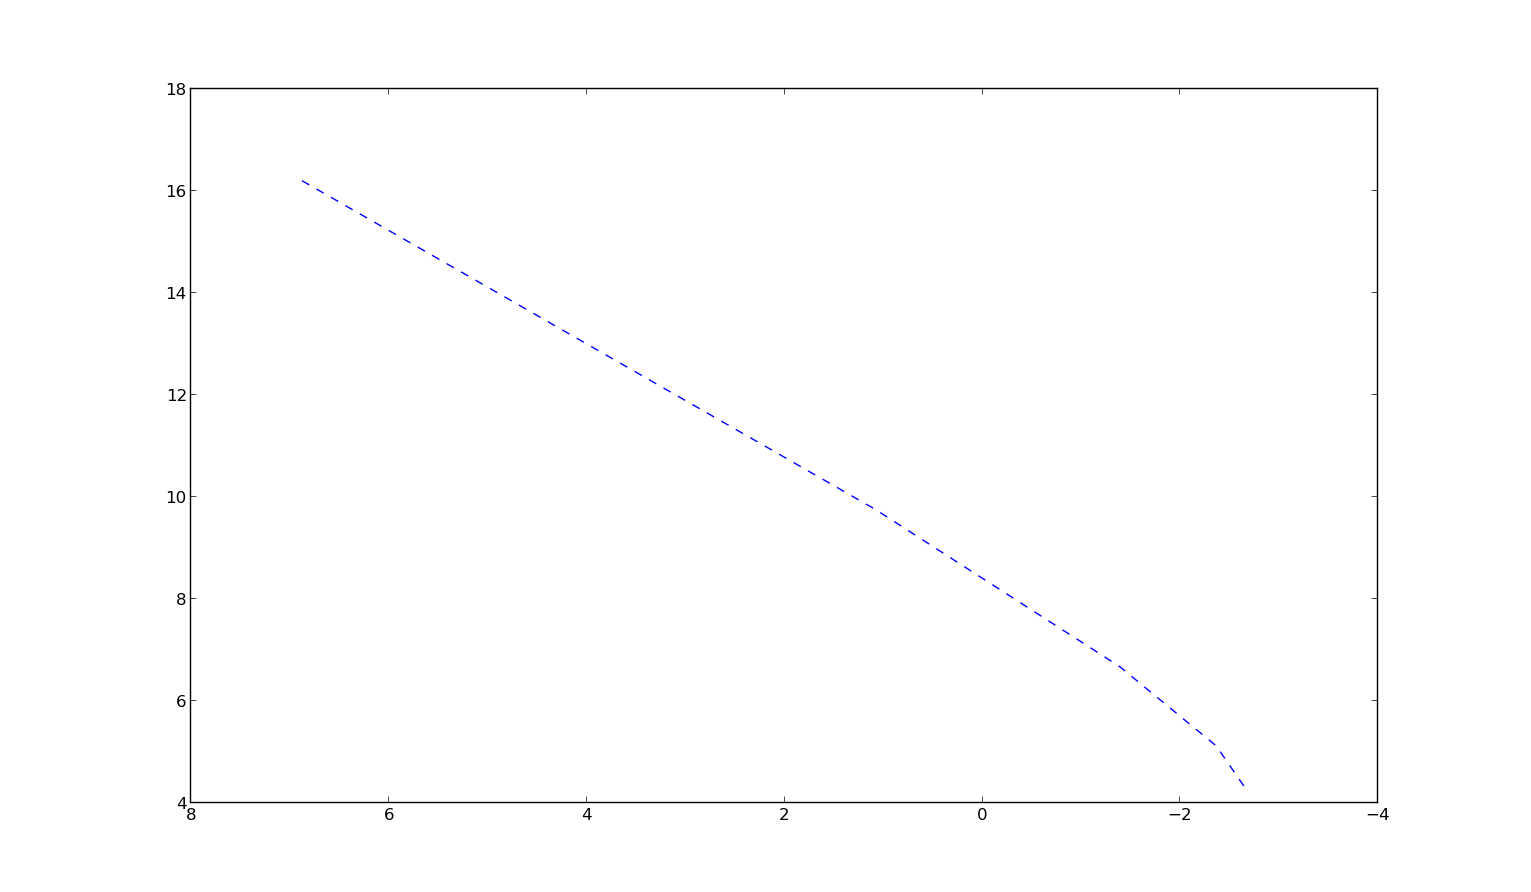
\includegraphics[scale=0.4]{LearningRate_3.png}
\[ w^{*} = \begin{bmatrix} 1.58164097\\ -0.93693741 \end{bmatrix}\]
for learning rate 0.3 \\

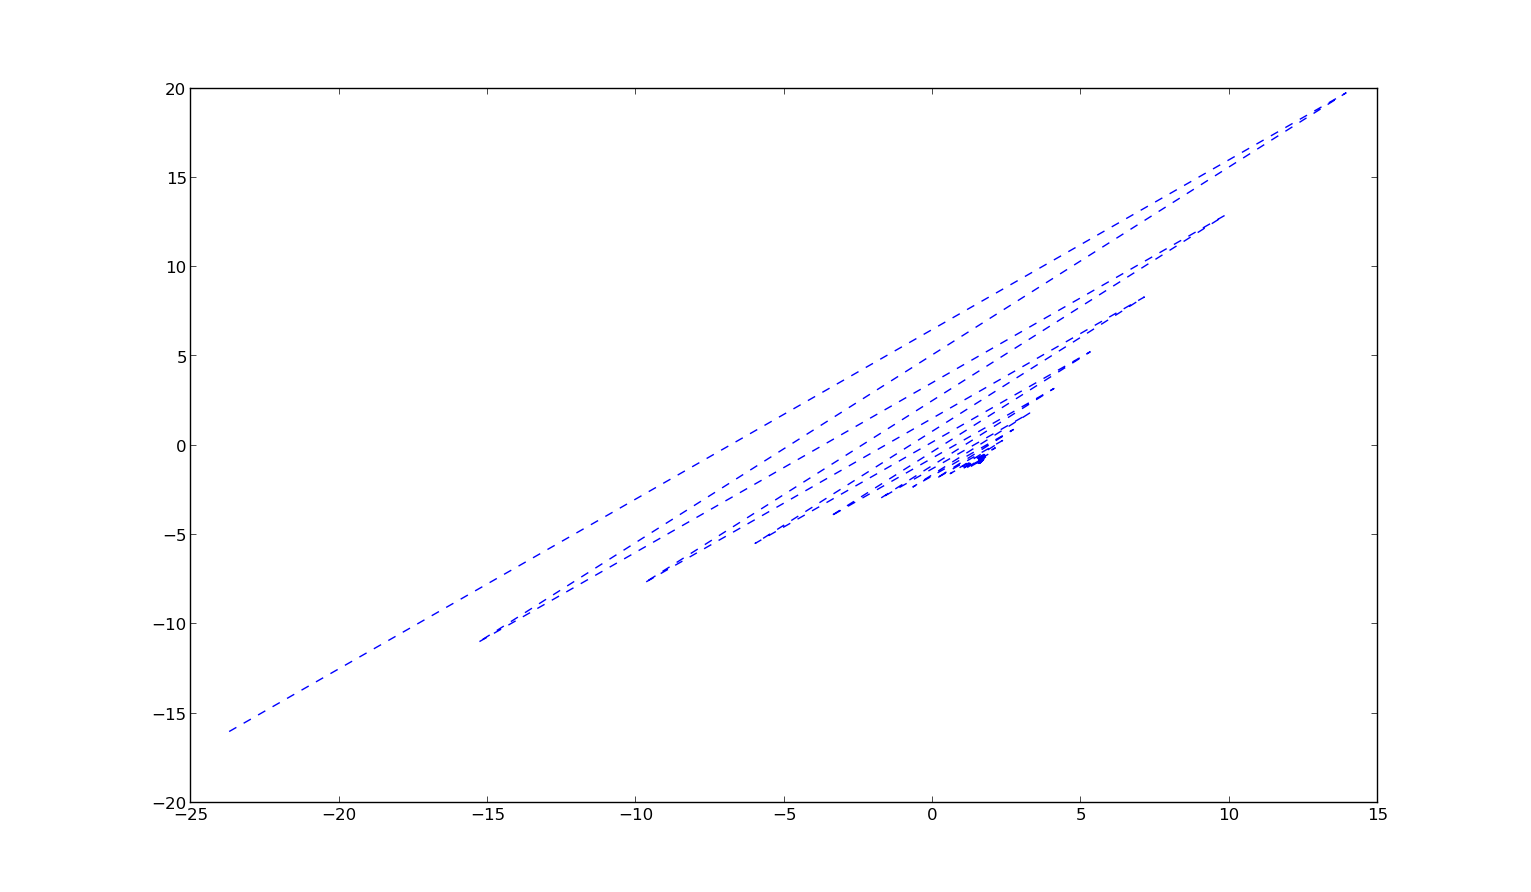
\includegraphics[scale=0.4]{LearningRate1.png}
\[ w^{*} = \begin{bmatrix} 1.5993919 \\ -0.95371617 \end{bmatrix}\]
for learning rate 1 \\

So we can see varying the learning rate does not have effect on the optimal value as they are \\
almost equal

\section{ (3.4) }
The LMS algorithm converges for 
$$0 < \eta < \frac{2}{\lambda_{max}} $$ 
where $\lambda_{max}$ is the largest eigen value of the correlation matrix.

Given the correlation matrix

$$
R_x =  
\left[ 
\begin{array}{cc}
1 & 0.5 \\ 
0.5 & 1 
\end{array} 
\right]
$$
The SVD of $R_x$ gives 1.5 as the the largest eigen value
This particular LMS problem will converge for 
$$ 0 < \eta <  \frac{2}{1.5} = 1.33 $$
\section{ (3.8) }
\subsection{ (a) }
Given 
$$ J(\pmb{w}) = \frac{1}{2}E[e^2(n)] = \frac{1}{2}E\left[(d(n)-\pmb{x}^T(n)\pmb{w})^2\right]$$

and E is a linear function,

$$ J(\pmb{w}) = \frac{1}{2} E\left[ d^2(n)-2\d(n) \pmb{x}(n)\pmb{w} + \pmb{x}(n)\pmb{w}^T\pmb{x}^T(n)\pmb{w} \right]$$
$$ = 
\frac{1}{2}  E\left[ d^2(n)\right] - 
\frac{1}{2}  2  E\left[d(n) \pmb{x}(n) \right]\pmb{w} + 
\frac{1}{2}  \pmb{w}^T  E\left[\pmb{x}(n) \pmb{x}^T(n) \right]\pmb{w}$$

$$ = 
\frac{1}{2}  \sigma_d^2 - 
\pmb{r}_{\pmb{x}d}^T\pmb{w} + 
\frac{1}{2}  \pmb{w}^T \pmb{R_x}  \pmb{w}$$
where
$$ \sigma_d^2 = E\left[ d^2(n)\right]$$
$$ \pmb{r}_{\pmb{x}d} = E\left[ \pmb{x}(n) d(n) \right]$$
$$ \pmb{R_x} = E\left[\pmb{x}(n) \pmb{x}^T(n) \right]$$
\subsection{ (b) }
Taking the gradient wrt to $\pmb{w}$ of  
$$
J(\pmb{w}) = 
\frac{1}{2}  \sigma_d^2 - 
\pmb{r}_{\pmb{x}d}^T\pmb{w} + 
\frac{1}{2}  \pmb{w}^T \pmb{R_x}  \pmb{w}$$
gives 
$$
\nabla J(\pmb{w}) = 
- \pmb{r}_{\pmb{x}d} + 
 \pmb{R_x}  \pmb{w} = g$$
 derivating again wrt $\pmb{w}$ we arrive at the Hessian
 $$  \pmb{H} =  \pmb{R_x}$$
 because of the transpose relation of the two $\pmb{w}$ terms and because 
 $$ \pmb{H}(f)(x)=\pmb{J}(\nabla f)(x)$$
\subsection{ (c) }
$$ e(n) = d(n) - \pmb{x}^T(n)\pmb{w}(n)$$
Hence
$$ \frac{\partial e(n)}{\partial \pmb{w}(n)} = -\pmb{x}(n) $$
the estimate of the gradient vector is then 

$$ \pmb{\hat g}(n) = -\pmb{x}(n)e(n) $$
and the steepest descent is described by
$$ \pmb{w}(n+1) = \pmb{w}(n) - \eta\pmb{g}(n)$$
we can formulate 
$$ \pmb{\hat w}(n+1) = \pmb{\hat w}(n) + \eta\pmb{x}(n)e(n) $$
which can be seen to equal 
$$\pmb{\hat w}(n) + \eta\pmb{x}(n)(d(n) - \pmb{x}^T(n)\pmb{w}(n)) $$
However, the $\pmb{R_x}$ term is still not accounted for.

\section{Code}
\begin{verbatim}
# -*- coding: utf-8 -*-
"""
Created on Sat Nov  7 12:33:53 2015

@author: poulastya
"""

import sympy
import numpy
import numpy as np
from numpy import *
from sympy import *
import math
import matplotlib.pyplot as plt
from matplotlib import *

"""
 Setting Initial weights at 20 and 30 and chaning the learning
rates
"""
w = np.matrix(([20],[30]))
l_r = 1
x = []
y = []

gradient = np.matrix(([l_r*(-0.8182+w.item(0)+0.8182*w.item(1))],

[l_r*(-0.354+w.item(1)+0.8182*w.item(0))]))

while (gradient.item(0) > 0.001 or gradient.item(0) < -0.001):
    w = w - gradient
    gradient = np.matrix(([l_r*(-0.8182+w.item(0)+0.8182*w.item(1))],
    
    [l_r*(-0.354+w.item(1)+0.8182*w.item(0))]))
    #print w    
    x.append(w.item(0))
    y.append(w.item(1))

print '####'
print w    

plt.plot(x,y,'b--')

plt.show()
\end{verbatim}
\end{document}